%\section{Problem Formulation and overview}
We will first analyze the safety issues in apprenticeship learning with a grid-world example. Then we will define the safety-aware apprenticeship learning (SafeAL) problem and give intuitions on how we solve it. 

%Given an $MDP\backslash R$ $M = (S, A, T, \gamma, D)$ and a set of m trajectories $\{\tau_0, \tau_1, ..., \tau_m\}$, now we define a set of atomic propositions $AP=\{'safe', 'unsafe', ...\}$ and use label function $L$ to label each $s\in S$ 'safe' or 'unsafe'. A specification $\Phi$ defines requirements on learnt policies. Especially, safety specification $\Phi$ formalized in PCTL can be in such forms: 

%\begin{eqnarray}
%\centering
%\Phi &=& [ \forall s^{(0)}\in S \Idge D(s^{(0)})\in (0, 1], s^{(0)}\models \phi]\label{eq:sec3_1}\\
%or\ \Phi &=& [ \sum_{s\in S} D(s^{(0)}) P_{=?|s^{(0)}}[\psi]\leq p^*]\label{eq:sec3_2}
%\end{eqnarray}
 
%(\ref{eq:sec3_1}) means that all initial states shall satisfy $\phi$. (\ref{eq:sec3_2}) means that the probability of initializing from some state and traveling along a trajectory that satisfies $\psi$ is smaller than $p^*$. Now that a policy $\pi^*$ has been learnt via apprenticeship learning algorithm, the safety of the learnt policy $\pi$ is defined as:

%\begin{definition}
%Policy $\pi$ for an MDP M is safe iff the DTMC D reduced from M and $\pi$ satisfies $\Phi$.
%\end{definition}
Assuming that there are some unsafe states
in an $MDP\backslash R$ $M = (S, A, T, \gamma, s_0)$. 
A safety issue means an agent following a learnt policy has a higher probability of entering those unsafe states than it should. There are multiple reasons that can give rise to this issue. First, it is possible that the expert policy itself has a high probability of reaching the unsafe states. Second, human experts often tend to perform only successful demonstrations that do not highlight the unwanted situations~\cite{shiarlis2016inverse}. This {\it lack of negative examples} in the training set results in the agent being unaware of the existence of those unsafe states.

%\vspace{-4mm}
\begin{figure}[!htb]
\centering
\subfigure[]{
	\begin{minipage}[c][1\width]{
	   0.4\textwidth}
	   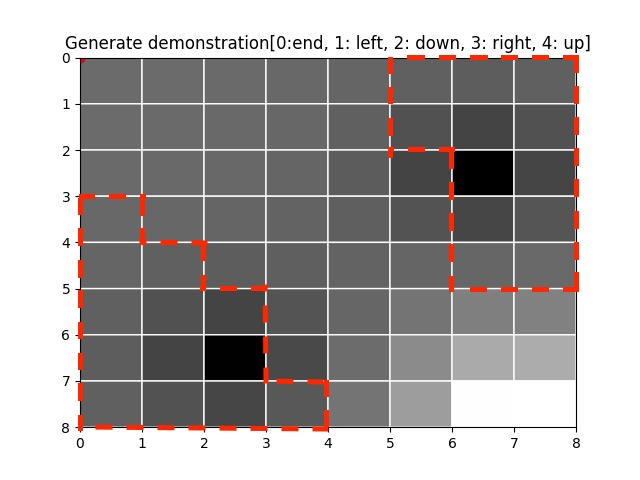
\includegraphics[width=1.\linewidth]{sec3_2.jpg}
	   \label{fig:sec3_2}
	\end{minipage}\hfill
}
\subfigure[]{
	\begin{minipage}[c][1\width]{
	   0.4\textwidth}
	   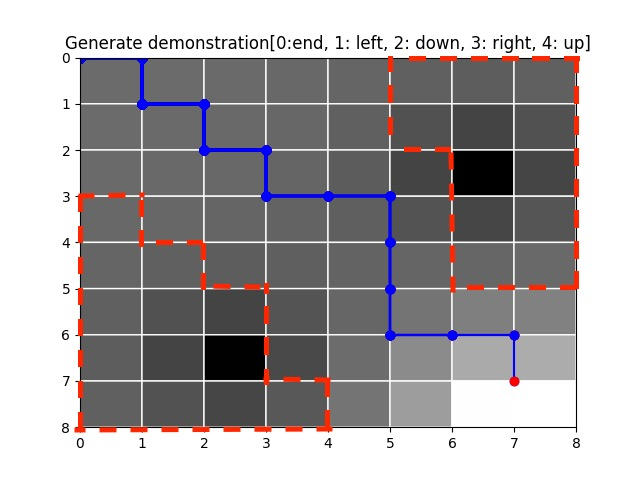
\includegraphics[width=1.\linewidth]{sec3_3.jpg}
	   \label{fig:sec3_3}
	\end{minipage}\hfill
}
\subfigure[]{
	\begin{minipage}[c][1\width]{
	   0.4\textwidth}
	   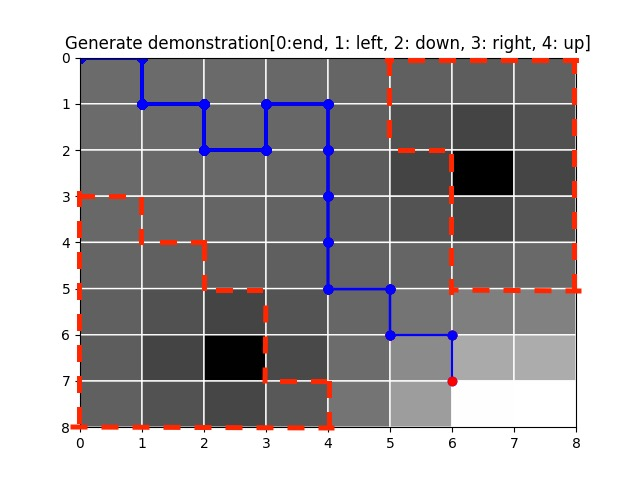
\includegraphics[width=1.\linewidth]{sec3_4.jpg}
	   \label{fig:sec3_4}
	\end{minipage}\hfill
}
\subfigure[]{
	\begin{minipage}[c][1\width]{
	   0.4\textwidth}
	   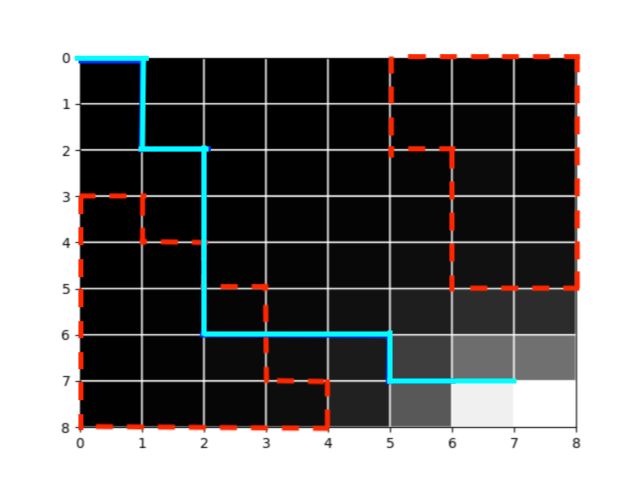
\includegraphics[width=1.\linewidth]{sec3_5.png}
	   \label{fig:sec3_5}
	\end{minipage}\hspace{0.012\linewidth}
}
\caption[Navigation task in gridworld]{
(a) The 8 x 8 gridworld. Lighter grid cells indicate relatively higher rewards while darker ones indicate lower rewards. It is regarded by the expert that the two black grid cells have the lowest rewards, while the two white ones constituting the goal area have the the highest rewards. The grid cells enclosed by red dashed lines are labelled as unsafe. (b) The blue line is the first representative trajectory that expert perform during demonstration. (c) The blue line is the second representative trajectory that expert perform during demonstration. (d) The rewards of the goal states have very high contrast against all other states. The difference between unsafe states and nearby states is so small that the agent has a high probability of performing a trajectory passing through the unsafe states as indicated by the cyan line.
}
\label{fig:grid_world1}
\end{figure}
%\vspace{-3mm}

We use a 8 x 8 grid world navigation example as shown in Fig.~\ref{fig:grid_world1} to illustrate this problem. The agent starts from the upper-left corner and moves from cell to cell until reaching the lower-right corner or a maximal step length $t<64$. Meanwhile, there are several cells labelled as unsafe enclosed by the red dashed lines shown near the upper-right and lower-left corners. These are regions that agent should avoid. 
In each time step, the agent can choose to stay in current cell or move to an adjacent cell. Due to stochasticity of the system, it has $30\%$ chance of moving randomly instead of moving accroding its decision. 
The expert knows the goal area, the unsafe area and the reward mapping on all states as shown in Fig.~\ref{fig:sec3_2}. For each state $s\in S$, the feature vector $f(s)$ consists of $4$ feature functions $f_i(s),\ i = 0, 1, 2, 3$. All of them are radial basis functions which respectively depend on the squared Euclidean distances between $s$ and the $4$ states with the highest or lowest rewards as shown in Fig.~\ref{fig:sec3_2}. In addition, a specification $\Phi$ formalized in PCTL is given to capture the safety requirement. In Eq.~\ref{eq:example-spec}, $p^*$ is the upper bound of the probability of reaching an unsafe state within $t=64$ steps and can be set by any value in $[0, 1]$ initially.
\begin{equation}
\Phi ::= P_{=?|s_0}[\true\ \until^{\leq t}\ \texttt{unsafe}]\leq p^*
\label{eq:example-spec}
\end{equation}

We extend the satisfaction relation $\models$ in PCTL and define that a policy $\pi\models\Phi$ if the initial state $s_0$ of the DTMC $M_\pi$ induced from MDP $M$ by policy $\pi$ satisfies the PCTL property in $\Phi$. We illustrate two scenarios in this simple example. The first simulates a setting with abundant expert demonstrations, i.e. $\mu_E$ is directly generated from the optimal policy $\pi_E$ with respect to the predetermined $\omega_E$ which results in the reward mapping in Fig.~\ref{fig:sec3_2}. In this case, the AL algorithm can accurately recover $\pi_E$. 
Model checking result shows that the probability of reaching an unsafe state by following the learnt policy, or the expert policy $\pi_E$ itself, is $11.7\%$. Hence, the specification is satisfied in this scenario. In the second scenario, which is more realistic, the expert follows $\pi_E$ but only performs a limited number of demonstrations which are all successful and safe. As indicated by the two representative (in blue) trajectories shown in Fig.~\ref{fig:sec3_3} and Fig.~\ref{fig:sec3_4}, $10,000$\footnote{This number is actually considered small for the size of this problem.} trajectories were used as expert demonstrations. 
The reward function that induces the learnt policy in this scenario is shown in Fig.~{\ref{fig:sec3_5}}.
Observe that only the goal area has been learnt whereas the agent is oblivious to the unsafe regions (treating them in the same way as other black cells). Indeed, probability of reaching an unsafe state within $64$ steps with this policy turns out to be $98\%$ (thus violating the safety requirement by a large margin).  
To make matters worse, the value of $p^*$ may be decided or revised after a policy has been learnt. In that case, even the original expert policy $\pi_E$ is unsafe, e.g., when $p^*=10\%$. 
Thus, we need to adapt the AL algorithm to account for this additional safety requirement. 
\begin{definition}
\textbf{The safety-aware apprenticeship learning (SafeAL) problem} is, given an $MDP\backslash R$, a set of $m$ trajectories $\{\tau_0, \tau_1, ..., \tau_{m-1}\}$ demonstrated by an expert, and a specification $\Phi$, to learn a policy $\pi$ that satisfies $\Phi$ and is $\epsilon$-close to the expert policy $\pi_E$.
\end{definition}
